\section{A Step by Step Process}

Real world reconstruction from scan data is a step by step process:

\begin{itemize}
\item Scanning and scans alignment => point set with or without normals (not covered by \cgal)
\item Outliers removal (if reconstruction method does not support outliers)
\item Point set simplification
\item Smoothing (if reconstruction method does not support noise)
\item Normals estimation and orientation (if not provided by scanner)
\item Surface reconstruction
\end{itemize}

This package provides algorithms for each step above.

A GUI demo (Windows only) allows to test each algorithm.


\subsection{Input}

Functions and classes of this package expect as input and output parameters range iterators over:

\begin{itemize}
\item 3D points
\item Normals (orientable 3D vectors)
\item 3D points with unoriented normals
\item 3D points with oriented normals
\end{itemize}

We provide several models of points and normals concepts, with different speed/space trade-offs:

\begin{itemize}
\item \ccRefIdfierPage{CGAL::Point_3<Geom_traits>} \\
\cgal\ regular 3D position.
\item \ccRefIdfierPage{CGAL::Vector_3<Geom_traits>} \\
\cgal\ regular 3D vector.
\item \ccRefIdfierPage{CGAL::Lightweight_vector_3<Geom_traits>} \\
3D vector allocated only if not (0,0,0).
\item \ccRefIdfierPage{CGAL::Orientable_normal_3<Geom_traits>} \\
Normal (oriented or not).
Inherits from \ccc{Vector_3<Geom_traits>} and contains an "is normal oriented?" flag.
\item \ccRefIdfierPage{CGAL::Point_with_normal_3<Geom_traits, Normal_3>} \\
3D position + normal.
\end{itemize}

For convenience, we provide also functions to read point sets from standard file formats:

\begin{itemize}
\item XYZ
\item OFF
\end{itemize}

\ccRefIdfierPage{CGAL::surface_reconstruction_read_xyz}  \\
\ccRefIdfierPage{CGAL::surface_reconstruction_read_off_point_cloud}  \\

Example:

\begin{ccExampleCode}
typedef CGAL::Exact_predicates_inexact_constructions_kernel Kernel;
typedef CGAL::Point_with_normal_3<Kernel> Point_with_normal;
std::deque<Point_with_normal> points;
char* filename = ...;

// Read the point set file in points[]
if(!CGAL::surface_reconstruction_read_off_point_cloud(filename,
                                                      std::back_inserter(points)))
{
  std::cerr << "Error: cannot read file " << filename << std::endl;
  return EXIT_FAILURE;
}
\end{ccExampleCode}


\subsection{Analysis}

The purpose of the analysis stage is to compute parameters for the next stages algorithms.

\begin{itemize}
\item Point set barycenter, bounding box, bounding sphere (provided by \cgal\ Principal Components Analysis package)
\item Average spacing to the K nearest neighbors
\end{itemize}

\ccRefIdfierPage{CGAL::centroid}  \\
\ccRefIdfierPage{CGAL::bounding_box}  \\
\ccRefIdfierPage{CGAL::average_spacing_3}  \\

Example:

\begin{ccExampleCode}
typedef CGAL::Exact_predicates_inexact_constructions_kernel Kernel;
typedef Kernel::FT FT;
typedef Kernel::Point_3 Point;
std::deque<Point> points = ...;
int nb_neighbors = 7;

typedef std::deque<Point>::iterator Iterator;
std::cerr << "Compute average spacing to knn ";
std::cerr << CGAL::average_spacing_3<Iterator,FT>(points.begin(), points.end(),
                                                  nb_neighbors) << "\n";
\end{ccExampleCode}


\subsection{Processing}

\subsubsection{Outliers Removal Methods}

\begin{itemize}
\item Outliers removal wrt average squared distance to the K nearest neighbors
\end{itemize}

\ccRefIdfierPage{CGAL::remove_outliers_wrt_avg_knn_sq_distance_3}  \\

% Insert image outliers_removal.jpg/eps
\begin{center}
    \label{Surface_reconstruction_3-fig-outliers_removal}
    % Image
    \begin{ccTexOnly}
        \includegraphics[width=0.9\textwidth]{Surface_reconstruction_3/outliers_removal} % omit .eps suffix
    \end{ccTexOnly}
    \begin{ccHtmlOnly}
        <img width="90%" border=0 src="./outliers_removal.jpg"><P>
    \end{ccHtmlOnly}
    % Title
    \begin{figure}[h]
        \caption{Outliers removal}
    \end{figure}
\end{center}

Example:

\begin{ccExampleCode}
typedef CGAL::Exact_predicates_inexact_constructions_kernel Kernel;
typedef Kernel::Point_3 Point;
std::deque<Point> points = ...;
int nb_neighbors = 7;
double threshold_percent = 50; // percentage of points to remove

// Remove outliers and put result in output iterator
std::deque<Point> output;
CGAL::remove_outliers_wrt_avg_knn_sq_distance_3(points.begin(), points.end(),
                                                std::back_inserter(output),
                                                nb_neighbors,
                                                threshold_percent);
\end{ccExampleCode}


\subsubsection{Point Set Simplification Methods}

\begin{itemize}
\item Point set simplification by clustering
\item Random point set simplification
\end{itemize}

\ccRefIdfierPage{CGAL::merge_epsilon_nearest_points_3}  \\
\ccRefIdfierPage{CGAL::random_simplification_points_3}  \\

% Insert image random_simplification.jpg/eps
\begin{center}
    \label{Surface_reconstruction_3-fig-random_simplification}
    % Image
    \begin{ccTexOnly}
        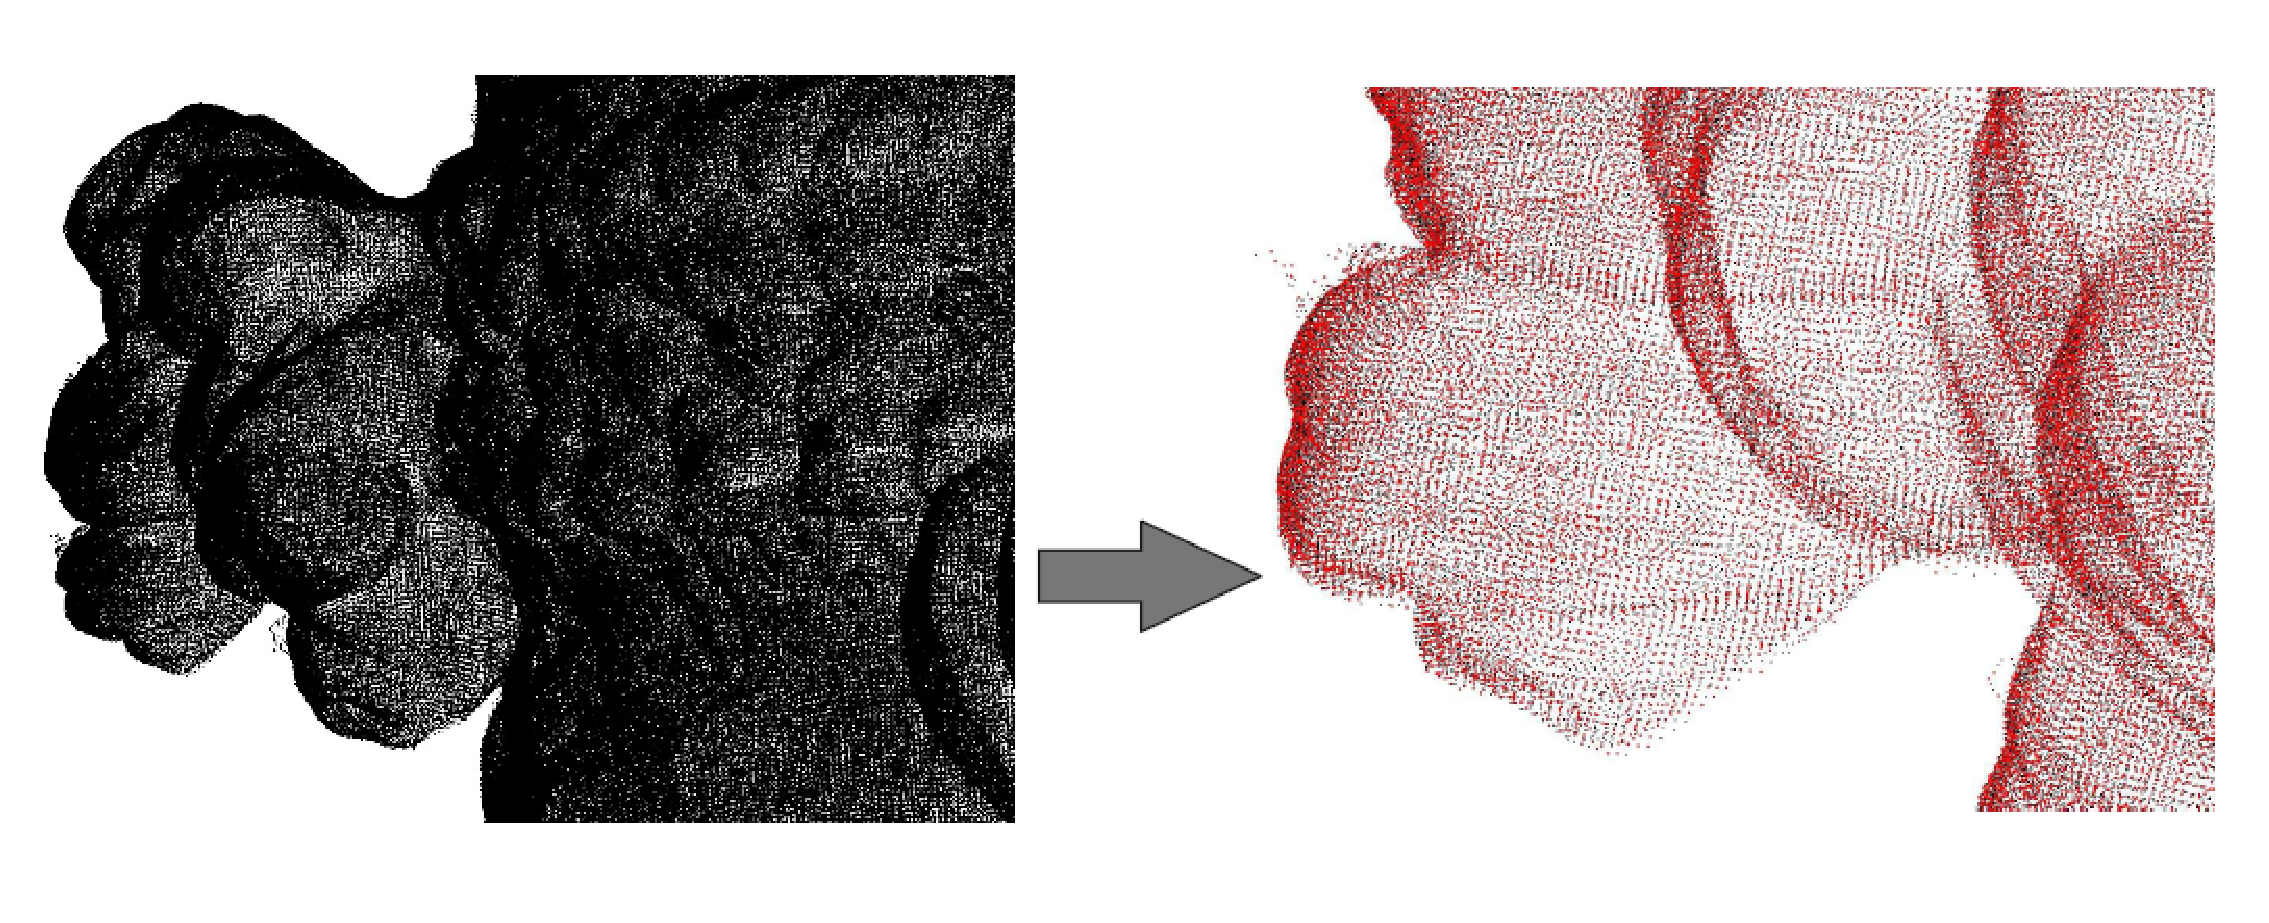
\includegraphics[width=0.9\textwidth]{Surface_reconstruction_3/random_simplification} % omit .eps suffix
    \end{ccTexOnly}
    \begin{ccHtmlOnly}
        <img width="90%" border=0 src="./random_simplification.jpg"><P>
    \end{ccHtmlOnly}
    % Title
    \begin{figure}[h]
        \caption{Random point set simplification}
    \end{figure}
\end{center}

Example:

\begin{ccExampleCode}
typedef CGAL::Exact_predicates_inexact_constructions_kernel Kernel;
typedef Kernel::Point_3 Point;
std::deque<Point> points = ...;
double epsilon = 0.001;

// Simplify point set by clustering and put result in output iterator
std::deque<Point> output;
CGAL::merge_epsilon_nearest_points_3(points.begin(), points.end(),
                                     std::back_inserter(output),
                                     epsilon);
\end{ccExampleCode}


\subsubsection{Smoothing Methods}

\begin{itemize}
\item Smoothing via Jet fitting over the K nearest neighbors + reprojection
\end{itemize}

\ccRefIdfierPage{CGAL::smooth_jet_fitting_3}  \\

% Insert image smoothing_jet_fitting.jpg/eps
\begin{center}
    \label{Surface_reconstruction_3-fig-smoothing_jet_fitting}
    % Image
    \begin{ccTexOnly}
        \includegraphics[width=1.0\textwidth]{Surface_reconstruction_3/smoothing_jet_fitting} % omit .eps suffix
    \end{ccTexOnly}
    \begin{ccHtmlOnly}
        <img width="100%" border=0 src="./smoothing_jet_fitting.jpg"><P>
    \end{ccHtmlOnly}
    % Title
    \begin{figure}[h]
        \caption{Point set smoothing}
    \end{figure}
\end{center}

Example:

\begin{ccExampleCode}
typedef CGAL::Exact_predicates_inexact_constructions_kernel Kernel;
typedef Kernel::Point_3 Point;
std::deque<Point> points = ...;
int nb_neighbors = 7;

// Smooth point set and put result in output iterator
std::deque<Point> output;
CGAL::smooth_jet_fitting_3(points.begin(), points.end(),
                           std::back_inserter(output),
                           nb_neighbors);
\end{ccExampleCode}


\subsubsection{Normals Estimation Methods}

\begin{itemize}
\item Normals estimation by Principal Components Analysis over the K nearest neighbors
\item Normals estimation by Jet fitting over the K nearest neighbors
\end{itemize}

\ccRefIdfierPage{CGAL::estimate_normals_jet_fitting_3}  \\
\ccRefIdfierPage{CGAL::estimate_normals_pca_3}  \\

% Insert image normal_estimation_pca.jpg/eps
\begin{center}
    \label{Surface_reconstruction_3-fig-normal_estimation_pca}
    % Image
    \begin{ccTexOnly}
        \includegraphics[width=0.9\textwidth]{Surface_reconstruction_3/normal_estimation_pca} % omit .eps suffix
    \end{ccTexOnly}
    \begin{ccHtmlOnly}
        <img width="90%" border=0 src="./normal_estimation_pca.jpg"><P>
    \end{ccHtmlOnly}
    % Title
    \begin{figure}[h]
        \caption{Normals estimation}
    \end{figure}
\end{center}


\subsubsection{Normals Orientation Methods}

\begin{itemize}
\item Normals orientation using a Minimal Spanning Tree \cite{cgal:hddms-srup-92}
\end{itemize}

\ccRefIdfierPage{CGAL::orient_normals_minimum_spanning_tree_3}  \\

% Insert image normals_orientation_mst.jpg/eps
\begin{center}
    \label{Surface_reconstruction_3-fig-normals_orientation_mst}
    % Image
    \begin{ccTexOnly}
        \includegraphics[width=0.9\textwidth]{Surface_reconstruction_3/normals_orientation_mst} % omit .eps suffix
    \end{ccTexOnly}
    \begin{ccHtmlOnly}
        <img width="90%" border=0 src="./normals_orientation_mst.jpg"><P>
    \end{ccHtmlOnly}
    % Title
    \begin{figure}[h]
        \caption{Normals orientation}
    \end{figure}
\end{center}


\subsection{Surface Reconstruction}

\subsubsection{Implicit Functions}

This package implements:

\begin{itemize}
\item Delaunay-based Poisson reconstruction \cite{Kazhdan06}
\item Algebraic Point Set Surfaces \cite{Guennebaud07}
\end{itemize}

\ccRefIdfierPage{CGAL::Poisson_implicit_function<ImplicitFctDelaunayTriangulation_3>}  \\
\ccRefIdfierPage{CGAL::APSS_implicit_function<GeomTraits, PointWithNormal_3>}  \\

% Insert image APSS.jpg/eps
\begin{center}
    \label{Surface_reconstruction_3-fig-APSS}
    % Image
    \begin{ccTexOnly}
        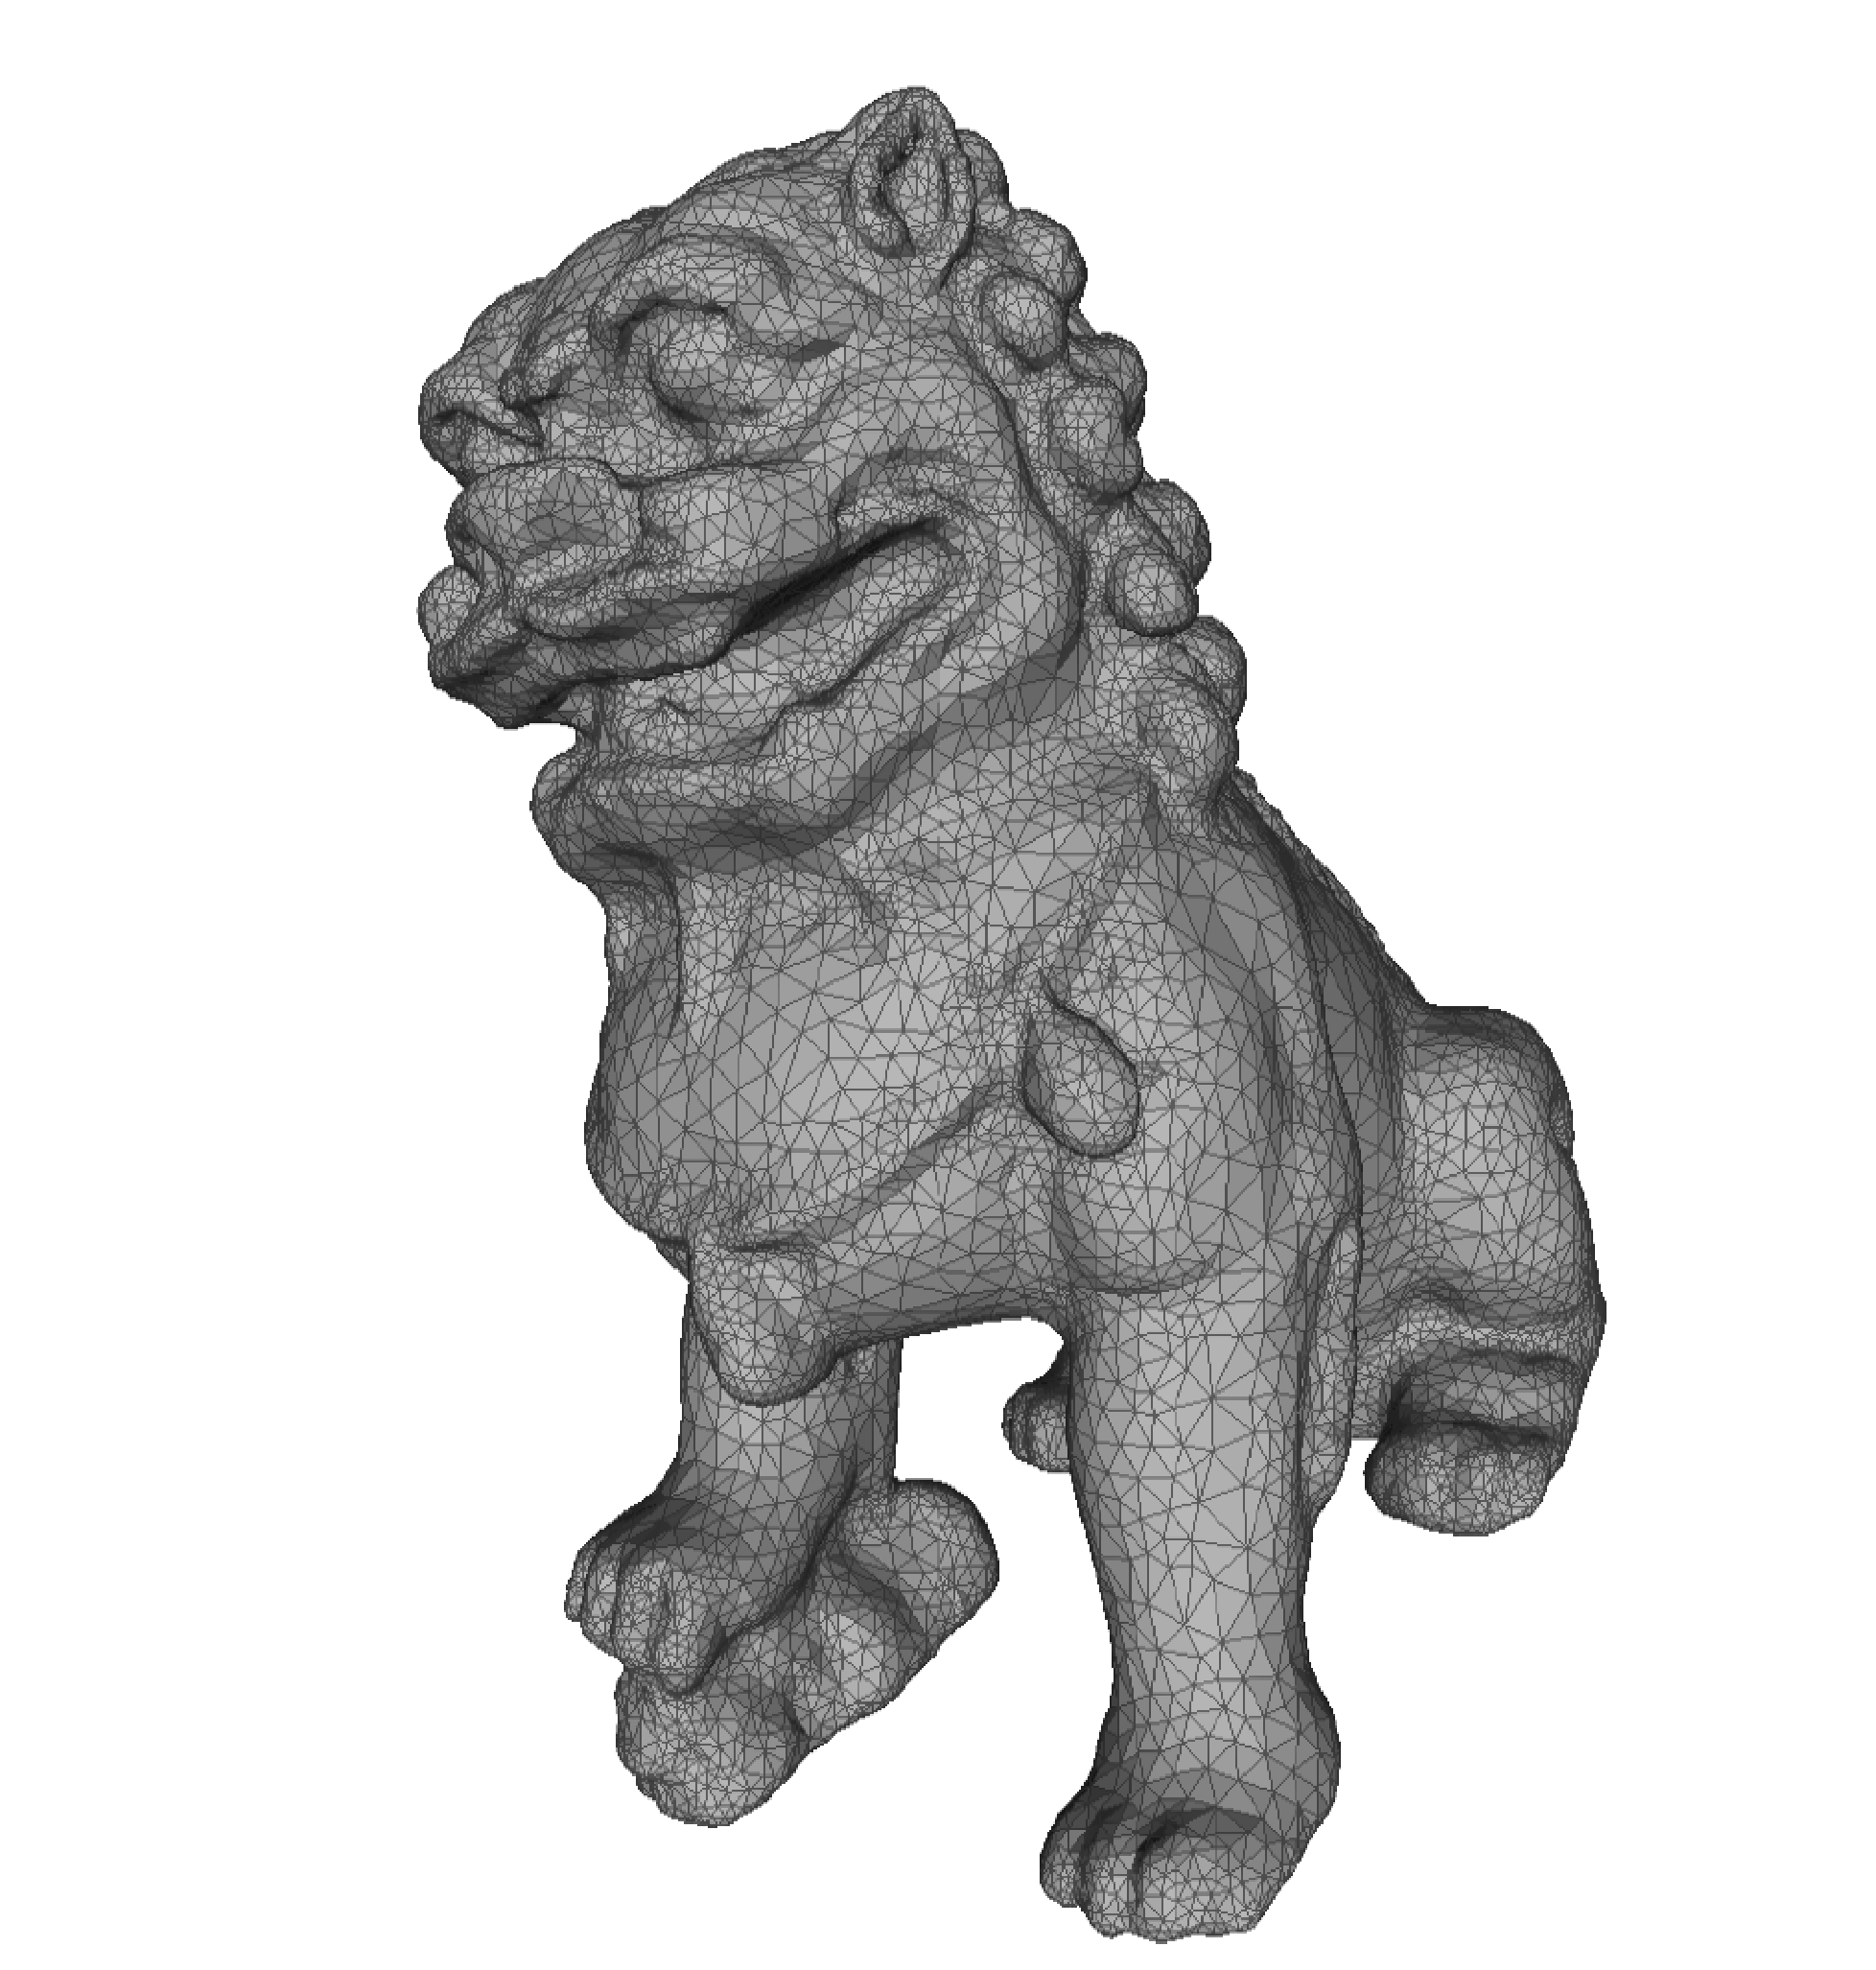
\includegraphics[width=0.5\textwidth]{Surface_reconstruction_3/APSS} % omit .eps suffix
    \end{ccTexOnly}
    \begin{ccHtmlOnly}
        <img width="50%" border=0 src="./APSS.jpg"><P>
    \end{ccHtmlOnly}
    % Title
    \begin{figure}[h]
        \caption{APSS reconstruction}
    \end{figure}
\end{center}


\subsubsection{Implicit Functions Contouring}

Implicit functions can be contoured to reconstruct a surface by:

\begin{itemize}
\item \cgal\ Surface Mesh Generator~\cite{cgal:ry-gsddrm-06,cgal:bo-pgsms-05}
\end{itemize}

\ccRefIdfierPage{CGAL::make_surface_mesh}  \\

The parameter \ccc{Tag} affects the behavior of \ccc{make_surface_mesh()}: \\
- \ccc{Manifold_tag}: the output mesh is guaranteed to be a manifold
surface without boundary.\\
- \ccc{Manifold_with_boundary_tag}: the output mesh is guaranteed to be
manifold but may have boundaries.\\
- \ccc{Non_manifold_tag}: the output mesh will be a polygon soup.

Example:

\begin{ccExampleCode}
typedef CGAL::Exact_predicates_inexact_constructions_kernel Kernel;
typedef CGAL::Surface_mesh_default_triangulation_3 STr;
typedef CGAL::Surface_mesh_complex_2_in_triangulation_3<STr> C2t3;
typedef CGAL::Implicit_surface_3<Kernel, Poisson_implicit_function> Surface_3;

Surface_3 surface =...; // Implicit function to contour

// Contour surface
STr tr; // 3D-Delaunay triangulation
C2t3 c2t3 (tr); // 2D-complex in 3D-Delaunay triangulation
CGAL::make_surface_mesh(c2t3, surface, ..., CGAL::Manifold_with_boundary_tag());
\end{ccExampleCode}


\subsection{Output}

\subsubsection{Point Set Output}

The output of the processing stage is a point set with normals.
For convenience, we provide functions to write point sets to standard file formats:

\begin{itemize}
\item XYZ
\item OFF
\end{itemize}

\ccRefIdfierPage{CGAL::surface_reconstruction_write_off_point_cloud}  \\
\ccRefIdfierPage{CGAL::surface_reconstruction_write_xyz}  \\

Example:

\begin{ccExampleCode}
typedef CGAL::Exact_predicates_inexact_constructions_kernel Kernel;
typedef CGAL::Point_with_normal_3<Kernel> Point_with_normal;
std::deque<Point_with_normal> points;
char* filename = ...;

// Save the point set to OFF file
if(!CGAL::surface_reconstruction_write_off_point_cloud(filename,
                                                       points.begin(), points.end()))
{
  std::cerr << "Error: cannot write file " << filename << std::endl;
  return EXIT_FAILURE;
}
\end{ccExampleCode}


\subsubsection{Surface Output}

The surface reconstructed by \ccc{make_surface_mesh()}
is required to be a model of the concept
\ccc{SurfaceMeshComplex_2InTriangulation_3},
a data structure able to represent a two dimensional
complex embedded in a three dimensional triangulation. \\
\ccc{SurfaceMeshComplex_2InTriangulation_3} defines the methods to traverse the reconstructed surface.

As examples, we provide functions to:

\begin{itemize}
\item write the reconstructed surface to standard OFF file format
\item convert the reconstructed surface to a polygon soup
\end{itemize}

\ccRefIdfierPage{CGAL::output_surface_facets_to_off}  \\
\ccRefIdfierPage{CGAL::surface_reconstruction_output_surface_facets}  \\

Example:

\begin{ccExampleCode}
typedef CGAL::Exact_predicates_inexact_constructions_kernel Kernel;
typedef CGAL::Surface_mesh_default_triangulation_3 STr;
typedef CGAL::Surface_mesh_complex_2_in_triangulation_3<STr> C2t3;
typedef CGAL::Implicit_surface_3<Kernel, Poisson_implicit_function> Surface_3;
typedef Kernel::Triangle_3 Triangle;

Surface_3 surface =...; // Implicit function to contour

// Contour surface
STr tr; // 3D-Delaunay triangulation
C2t3 c2t3 (tr); // 2D-complex in 3D-Delaunay triangulation
CGAL::make_surface_mesh(c2t3, surface, ...);

// Convert reconstructed surface to a triangles soup
std::deque<Triangle> triangles;
CGAL::surface_reconstruction_output_surface_facets(c2t3, std::back_inserter(triangles));
\end{ccExampleCode}






